\documentclass{beamer}
\usetheme{Madrid} % You can choose other themes like Warsaw, Berlin, etc.
\usepackage{graphicx}
\usepackage[table]{xcolor} % For colored table cells
\usepackage{tabularx}     % For tables with specified width
\usepackage{array}        % For advanced column formatting in tables

% --- WIRE COLORS DEFINED BASED ON USER'S RGB VALUES FOR THE 16 PINS ---
% Mapping based on the order of pins provided by the user:
% 1. 5V, 2. GND, 3. IO12, 4. IO13, 5. IO15, 6. IO14, 7. IO2, 8. IO4
% 9. 3V3, 10. IO16, 11. IO0, 12. GND, 13. VCC, 14. VOR, 15. VOT, 16. GND

\definecolor{clrPin1}{HTML}{010067}  % For 5V
\definecolor{clrPin2}{HTML}{9E008E}  % For GND (first instance)
\definecolor{clrPin3}{HTML}{FFE502}  % For GPIO 12 (was IO12)
\definecolor{clrPin4}{HTML}{005F39}  % For GPIO 13 (was IO13)
\definecolor{clrPin5}{HTML}{95003A}  % For GPIO 15 (was IO15)
\definecolor{clrPin6}{HTML}{FF937E}  % For GPIO 14 (was IO14)
\definecolor{clrPin7}{HTML}{001544}  % For GPIO 2 (was IO2)
\definecolor{clrPin8}{HTML}{91D0CB}  % For GPIO 4 (was IO4)

\definecolor{clrPin9}{HTML}{0E4CA1}  % For 3.3V
\definecolor{clrPin10}{HTML}{007DB5} % For GPIO 16 (was IO16)
\definecolor{clrPin11}{HTML}{6A826C} % For GPIO 0 (was IO0)
\definecolor{clrPin12}{HTML}{00AE7E} % For GND (second instance)
\definecolor{clrPin13}{HTML}{C28C9F} % For VCC
\definecolor{clrPin14}{HTML}{008F9C} % For UOR (was VOR)
\definecolor{clrPin15}{HTML}{5FADB2} % For UOT (was VOT)
\definecolor{clrPin16}{HTML}{FF029D} % For GND (third instance)


\title[IntelliGaze]{IntelliGaze: A Wearable AI Camera System}
\subtitle{Circuit Diagram and Pinout Connections}
\author[Seyam  , Eftekhar  , Mim  , Mahin  , Muntasir  ]{
    Touhidul Alam Seyam (230240003)\\ 
    Eftakar Uddin (230240004) \\ 
    Tasmim Akther Mim (230240025) \\ 
    Shafiul Azam Mahin (230240022) \\ 
    Muntasir Rahman (230240002)
}
\date{\today}
\institute{
    Microprocessor Lab \\ 
    Future Professor Radiathun Tasnia,\\ Junior Lecturer, \\ BGC Trust University Bangladesh
}

\begin{document}

% --- SLIDE 1: Title and Project Info ---
\begin{frame}
  \titlepage
\end{frame}


% --- SLIDE 2: Circuit Diagram ---
\begin{frame}{ESP32-CAM to ESP32-CAM-MB Wiring Diagram}
  \begin{figure}
    \centering
    \includegraphics[width=0.9\textwidth, keepaspectratio]{esp32_wiring_diagram.png}
    \caption{ESP32-CAM Pinout Diagram (Image Credit: RandomNerdTutorials.com).}
  \end{figure}
\end{frame}

% --- SLIDE 3: Pinout Table (Part 1) ---
\begin{frame}{Pinout Connections (Part 1)}
  \frametitle{ESP32-CAM to ESP32-CAM-MB Pinout (1/2)}
  \renewcommand{\arraystretch}{1.4} % Adjusted row height slightly for two lines
  \begin{tabularx}{\textwidth}{|>{\centering\arraybackslash}p{4cm}|>{\centering\arraybackslash}X|>{\centering\arraybackslash}X|>{\centering\arraybackslash}X|}
    \hline
    \textbf{Wire Color} & \textbf{Voltage} & \textbf{ESP32-CAM Pin} & \textbf{ESP32-CAM-MB Pin} \\
    \hline
    \colorbox{clrPin1}{\textcolor{white}{\shortstack{\bfseries 5V}}} & 5V & 5 V & 5V \\
    \hline
    \colorbox{clrPin2}{\textcolor{white}{\shortstack{\bfseries GND}}} & 0 V & GND & GND \\
    \hline
    \colorbox{clrPin3}{\textcolor{black}{\bfseries GPIO 12}} & 3.3V & GPIO 12 & GPIO 12 \\
    \hline
    \colorbox{clrPin4}{\textcolor{white}{\bfseries GPIO 13}} & 3.3V & GPIO 13 & GPIO 13 \\
    \hline
    \colorbox{clrPin5}{\textcolor{white}{\bfseries GPIO 15}} & 3.3V & GPIO 15 & GPIO 15 \\
    \hline
    \colorbox{clrPin6}{\textcolor{black}{\bfseries GPIO 14}} & 3.3V & GPIO 14 & GPIO 14 \\
    \hline
    \colorbox{clrPin7}{\textcolor{white}{\bfseries GPIO 2}} & 3.3V & GPIO 2 & GPIO 2 \\
    \hline
    \colorbox{clrPin8}{\textcolor{black}{\bfseries GPIO 4}} & 3.3V & GPIO 4 & GPIO 4 \\
    \hline

  \end{tabularx}
\end{frame}

% --- SLIDE 4: Pinout Table (Part 2) ---
\begin{frame}{Pinout Connections (Part 2)}
  \frametitle{ESP32-CAM to ESP32-CAM-MB Pinout (2/2)}
  \renewcommand{\arraystretch}{1.4} % Adjusted row height slightly for two lines
  \begin{tabularx}{\textwidth}{|>{\centering\arraybackslash}p{4cm}|>{\centering\arraybackslash}X|>{\centering\arraybackslash}X|>{\centering\arraybackslash}X|}
    \hline
    \textbf{Wire Color} & \textbf{Voltage} & \textbf{ESP32-CAM Pin} & \textbf{ESP32-CAM-MB Pin} \\
    \hline
    \colorbox{clrPin9}{\textcolor{white}{\bfseries 3.3V}} & 3.3V & 3.3V & 3.3V \\
    \hline
    \colorbox{clrPin10}{\textcolor{white}{\bfseries GPIO 16}} & 3.3V & GPIO 16 & GPIO 16 \\
    \hline
    \colorbox{clrPin11}{\textcolor{white}{\bfseries GPIO 0}} & 3.3V & GPIO 0 & GPIO 0 \\
    \hline
    \colorbox{clrPin12}{\textcolor{white}{\bfseries GND}} & 0V & GND & GND \\
    \hline
    \colorbox{clrPin13}{\textcolor{black}{\bfseries VCC}} & 3.3V / 5V & VCC & VCC \\
    \hline
    \colorbox{clrPin14}{\textcolor{white}{\bfseries UOR}} & 3.3V & UOR (GPIO3) & UOR (GPIO3) \\
    \hline
    \colorbox{clrPin15}{\textcolor{black}{\bfseries UOT}} & 3.3V & UOT (GPIO1) & UOT (GPIO1) \\
    \hline
    \colorbox{clrPin16}{\textcolor{white}{\bfseries GND}} & 0V & GND & GND \\
    \hline

  \end{tabularx}
\end{frame}
% --- SLIDE: Camera Data Pins ---
\begin{frame}{Used GPIO Pins: Camera Data}
  \frametitle{Camera Data Pins (Y2-Y9)}
  \begin{figure}
    \centering
    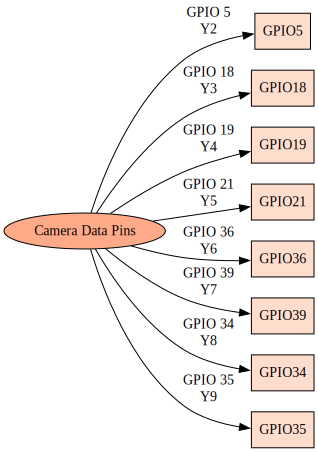
\includegraphics[width=0.40\textwidth]{camera_data_pins.png}
    \caption{GPIO pins used for camera data signals (Y2-Y9).}
  \end{figure}
\end{frame}

% --- SLIDE: Camera Control Pins ---
\begin{frame}{Used GPIO Pins: Camera Control}
  \frametitle{Camera Control Pins}
  \begin{figure}
    \centering
    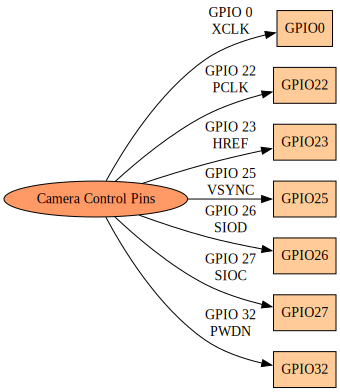
\includegraphics[width=0.40\textwidth]{camera_control_pins.png}
    \caption{GPIO pins used for camera control (clock, sync, I2C, power-down).}
  \end{figure}
\end{frame}

% --- SLIDE: Serial Communication Pins ---
\begin{frame}{Used GPIO Pins: Serial Communication}
  \frametitle{Serial Communication Pins}
  \begin{figure}
    \centering
    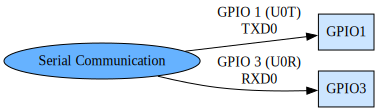
\includegraphics[width=0.7\textwidth]{serial_comm.png}
    \caption{GPIO pins used for UART serial communication.}
  \end{figure}
\end{frame}

% --- SLIDE: Power Pins ---
\begin{frame}{Used GPIO Pins: Power}
  \frametitle{Power Pins}
  \begin{figure}
    \centering
    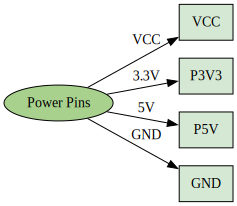
\includegraphics[width=0.6\textwidth]{power_pins.png}
    \caption{Power supply pins used (5V, 3.3V, VCC, GND).}
  \end{figure}
\end{frame}

% --- SLIDE: Unused/Available Pins ---
\begin{frame}{Other Available GPIO Pins}
  \frametitle{Unused GPIO Pins Available for Custom Use}
  \begin{itemize}
    \item \textbf{GPIO 2}
    \item \textbf{GPIO 4} (On-board flash LED on AI\_THINKER)
    \item \textbf{GPIO 12}
    \item \textbf{GPIO 13}
    \item \textbf{GPIO 14}
    \item \textbf{GPIO 15}
    \item \textbf{GPIO 16}
  \end{itemize}
\end{frame}

\end{document}